\section*{Analysis}
\label{Analyse}
%
Based on the results presented in the previous section it is possible to analyze how well a fit the BTL-model is.\blankline
%
According to the total number of possible violations namely 129, it seems that the BTL-model is a good fit, especially according to the low number of WST violations of which there where only two. Because the BTL-model sufficiently describe the data it is possible to view the original ordinal data as ratio data where each of the 10 sounds have their own scale value. Furthermore the resultant p-value of 0.3725, found with the Chi-square test, confirms the goodness of the fit because the p-value is above the significant level set at 0.1.

To signify what the analysis shows, the scale values for each sound and their respective confidence intervals are plotted in \autoref{fig:Confidens}. 
%
\begin{figure}[H]
\centering
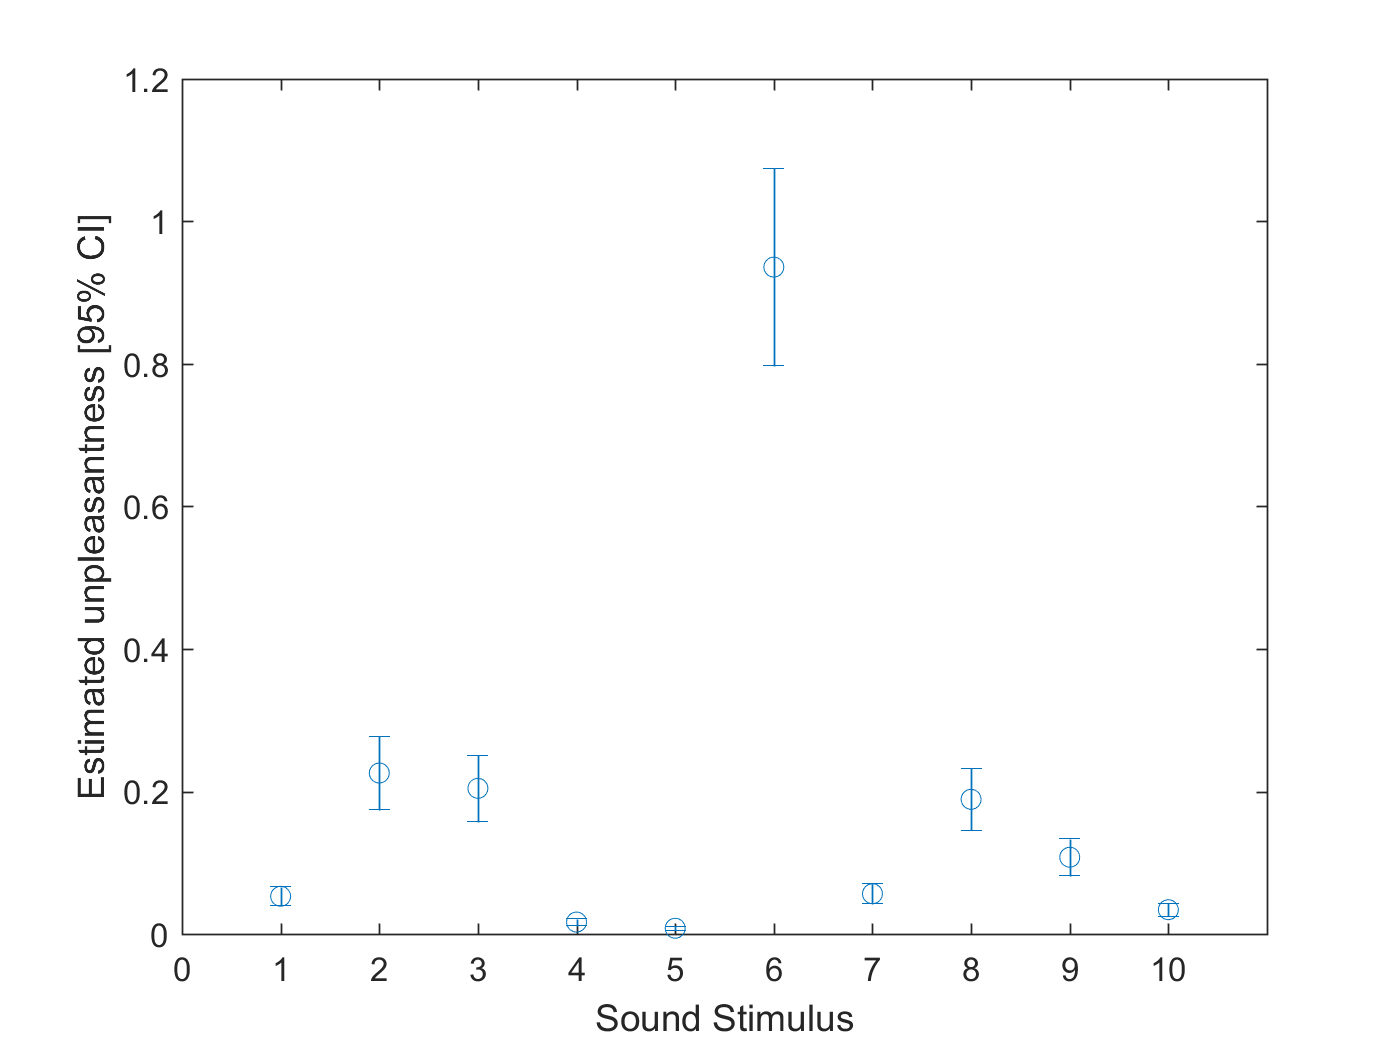
\includegraphics[width = 0.90\textwidth]{Figure/Confidens.png} 
\caption{Scale values and 95 \% confidence intervals for each of the 10 sounds.}
\label{fig:Confidens}
\end{figure}
\noindent 
%
From \autoref{fig:Confidens} it is clear that the scale value for sound number six is significantly different from all other values, i.e. the confidence intervals for sound number six does not overlap with the remaining nine confidence intervals. Based on \autoref{fig:Confidens}, there are some indications that the remaining nine sounds are split into two groups. The first group, which is the group with the highest ratings except from sound six, consists of sound number two, three, eight, and nine. These four sound numbers or scale values are not significantly different from each other, but they are significantly different from both sound six and the other group. The other group consists of sound number one, four, five, seven, and ten which got the lowest rankings, thus are the sounds which are less unpleasant compared to the others.   



